\title{Лекции по экологии}
\chapter{Лекция 4}

Лимитирующий фактор (условие) - любой фактор или условие среды, приближенное к пределу устойчивости (толлерантности) или превышающее его.

Закон Либиха (минимума) - при стационарном состоянии экологических фаторов лимитирующим будет тот из них, значение которого близко к необходимому минимуму.

\begin{figure}[H]
	\center{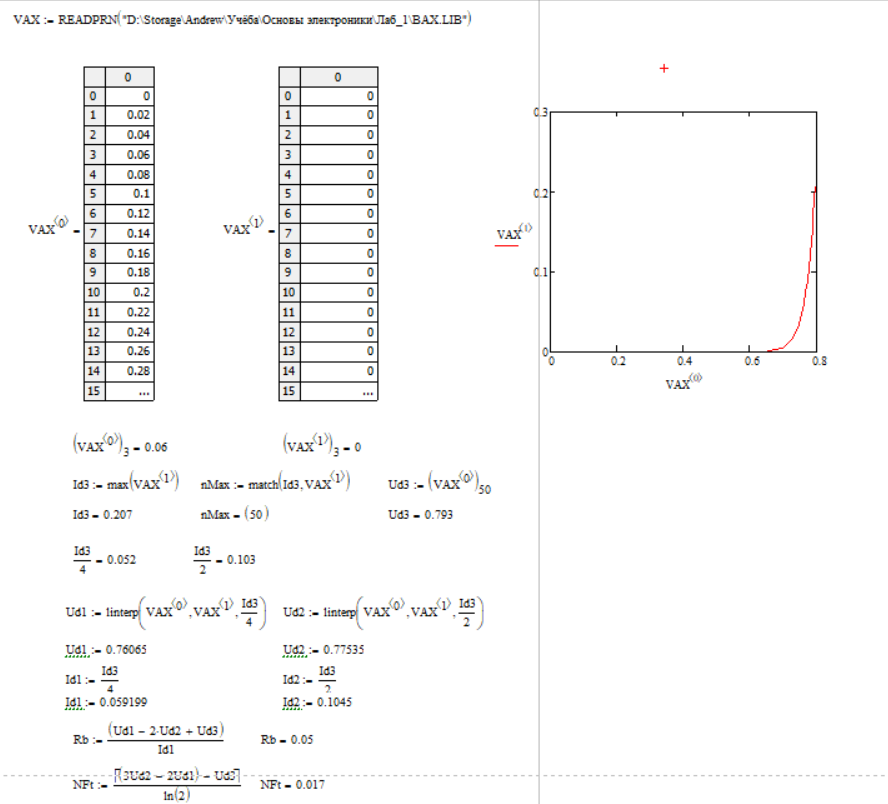
\includegraphics[scale=1.5]{0}}
	\caption{бочка Либиха}
\end{figure}

Заколн толерантности Шелфорда - любой живой организм имеет определённый верхний и нижний предел устойчивости к любому экологическому фактору.

Эврибионты - организмы, выдерживающие большие изменения фактора без существенных изменений процессов жизнедеятельности.

Стенобионты - оранизмы с узким пределом выносливости по отношению к тому же фактору.

Взаимодействие факторов: \\
Аддитивность - суммирование эффекторв влияния различных факторов.\\
Синергизм - обоюдное усиление действия различных  факторов.\\
Антогенизм - взаимное ослабление действия различных факторов.\\

Экологическая ниша - совокупность всех факторов среды, в пределах которых возможно существование видов в дикой природе.

Виды экологических ниш:\\
1. Пространственная экологичесая ниша - места обитания организмов.\\
2. Трофическая экологическая ниша - характеризует особенностями жизни организма в данной нише.\\

Экологические ниши организма определяются как n-мерный гиперобъем, охватывающий полный диапазо условий, в которых организм может уверенно воспроизводить себя.

Фундаментальная (потенциальная) ниша - совокупность оптимальных условий для организма.

Фактическая экономическая ниша - экономическая ниша в естественных условиях.

\section{Абиотический факторы среды}
Абиотический фактор среды - фактор неживой природы. Окружающие факторы, которые не зависят от человека (климат, погода, гравитация и тд...).
\subsection{Солнечная радиация}
Компоненты солнечной радиации - ультрафиолетовое, видимое и инфракрасное излучение. Видимое - используется растениями для выработки кислорода и для работы органов зрения. Инфракрасные лучи - переносят тепло. Ультрафиолетовые лучи - в случае людей используются для выработки витамина D, черезмерное облучение может привести к ускоренному старению и ожогам кожного покрова. 

Фотопериод - длина светового дня, определяет время года. Около 12 часов - на экваторе, чем дальше - тем меньше. 

Самый важный процесс, происходящий благодаря солнечному свету - фотосинтез, процесс выработки кислорода растениями.
$CO_{2} + H_{2}O \rightarrow C_{2}H_{12}O_{6} + O_{2}$

\subsection{Температура}
Связана с солнечным излучением и геотермальными источниками. Тепло на Земле определяется углом падения солнечных лучей. В летний период возможно температурная инверсия - теплые атмосферные слои опускаются ближе к поверхности. Для живых организмов оптимальная температура - от 0 до 25 градусов. Организмы могут регулировать температуру, эктотермы - от внешних истоников, экзотермы - от химических реакций внутри организма.

Эффективная температура - температура, оптимальная для жизни определённых видов животных и растений. Организмы могут адаптироваться к высоким и низким температурам. При адаптации к низком температурам, животные могут либо входит в состояние анабиоза, либо активно вырабатывать тепло, чтобы не допустить замерзание организма.

Правило Бертмана - чем быстрее животное и чем компактнее его тело, тем легче ему поддерживать температуру.

Правило Альмана - в более холодных областях у животных короче выступающие части тела.

Как для эктотермов, так и для эндотермов характерно наличие оптимальной температуры.

\subsection{Вода}
Вода выступает в качестве важнейшего экологического фактора. Работает в качестве компонента организма и среды обитания. Работает в виде натурального теплового аккумулятора, накапливая тепло летом и отдавая его зимой. Влажность и осадки являются факторами, влияющими на экологические условия. 

Все способы адаптации организма к содержанию воды в окружающей среде связаны с большим количеством процессов, компонентом которых является вода, протекающих внутри организма. Вода является основой протоплазмы и большей части жидкостей в организме. Ипользуется в капиллярной системе для транспортировки крови по телу. Испарение воды позволяет охладить организм. 

\subsection{Атмосферные газы и атмосферное давление}

Атмосфера - газовая оболочка, окружающая планету. В состав атмосферы входят азот, кислород, углекислый газ и другие газы. В атмосфере также содержатся газы техногенного происхождения. Атмосфера работает в качестве буфера между Землей и космосом. Большая часть опасных излучений задерживается атмосферой. 

Озоновый слой - слой озона, поглощающий смертельные для живых организмов лучи, приходящие из космоса.

Атмосферное давление - давление атмосферы. Чем дальше от поверхности, тем меньше давление. Давление атмофсеры может колебаться в зависимости от массы воздушных масс. Воздух обеспечивает работу слухового аппарата, работающего за счёт восприятия колебаний воздуха. Атмофсера является защитой от космических объектов, сгорающих в ней до попадания на поверхность. Атмосфера является основой климата. Атмосфера является основным источником азота, явлющегося однм из самых важных элементов во многих биологических процессов. Циклон - воздушный вихрь, вращающийся вокруг вертикальной оси. Диаметр циклона может достигать нескольких тысяч километров.

\chapter{Лекция 5}
\section{Биотические факторы среды}
Биотические факторы - совокупность влияния жизнедеятельности одних организмов на другие. Иначе данные факторы называются факторами живой природы.

Классификация биотических факторов по происхождению:
\begin{itemize}
\item зоогенные факторы - факторы взаимодействия между животными организмами.
\item фитогенные факторы - факторы, обусловленные взаимодействием между растительными организмами.
\item антропогенные факторы - факторы, обусловленные взаимодействием человека на окружающую среду, у некоторых видов является причиной возникновения социальной иерархии.
\end{itemize}

Классификация зоогенных факторов:
\begin{itemize}
\item гомотипическая реакция - взаимодействие между особями одного вида.
\begin{itemize}
	\item групповой эффект - выражается в повышении жизнеспособности организмов при их объединении в группы, может наблюдаться ускорение развитие и появление биологических особенностей.
	\item массовый эффект - вызывается негативными изменениями в среде обитания при превышении популяции особи критического уровня.
	\item внутривидовая конкуренция - конкуренция между особями одного вида за ресурсы.
\end{itemize}
\item гетеротипическая реакця - взаимодействие между особями разных видов.
\begin{itemize}
	\item нейтрализм - взаимоотношение между видами, занимающими одну территорию, но не оказывающими влияния друг на друга.
	\item хищничество - уничтожение одним видом организмов другого для потребления в пищу.
	\item паразитизм - взаимодействие, при котором один из видов существует за счёт органического вещества, получаемого от другого организма. Выделяют два вида паразитов - эндопаразиты, существуют внутри организма хозяина, и эктопаразиты, существуют вне организма хозяина.
	\item межвидовая конкуренция - взаимодействие двух и более видов организмов, стремящихся получить один и тот же ресурс. Прямая конкуренция - агрессивное столкновение за ресурс. Косвенная конкуренкция - опосредование столкновение за ресурс.
	\item симбиоз - взаимоотношение разных видов, при котором несколько организмов получают взаимную выгоду, способствующую их росту и выживанию. Частный случай симбиоза - мутуализм. Это вид взаимоотношений при котором каждый организм получает выгоду, при этом для хотя бы одного вида организма присутсвие партнёра является жизненеобходимым.
	\item комменциализм (нахлебничество) - вид взаимоотношений, при которых только один из партнёров получает выгоду, не нанося ущерба другому и не принося пользы.
\end{itemize}
\end{itemize}
Данные подгруппы называются реакциями.

Классификация фитогенных факторов:
\begin{itemize}
\item прямые
\begin{itemize}
\item механические взаимодействия
\item физиологические (паразитические, симбиоз, мутуализм)
\end{itemize}
\item косвенные
\begin{itemize}
\item световое окружение
\item создание подстилающей поверхности
\end{itemize}
\end{itemize}

Антропогенные факторы - прямые или косвенные воздействия человека на среду, вызывающее изменение экосистем и влияющее на здоровье населения.

Прямые факторы - непосредственное воздействие человека (охота, рыбалка, вырубка лесов).\\
Косвенные - связаны с деятельностью человека.

Классификация:\\
Физические - электромагнитные поля и излучения, радиация, шумовое загрязнение, тепловое загрязнение.\\
Химические - тяжёлые металлы, диоксиды и их производные, пестициды, ПАУ (полициклические ароматические углеводороды), нитриты и нитраты.\\


Принцип Олли - для каждого вида существует оптимальный размер группы и оптимальная плотность популяции, как и перенаселённость, так и недонаселённость оказывают неблагоприятное влияние.

Закон конкурентного исключения (Закон Гаузе) - победителем в конкурентной борьбе оказывается тот вид, который в данной экологической обстановке имеет хотя бы небольшие преимущества перед другим видом. А следовательно - большую приспособленность к условиям окружающей среды.

\chapter{Лекция 6}
\section{Антропогенные факторы}
Эффект биоаккумуляции - увеличение концетрации загрязнителей на каждом последующем уровне в трофической цепи.

Воздействие антропогенных факторов:\\
на молекулярном уровне - хромосомные и генные повреждения\\
на клеточном уровне - снижение иммунитета\\
на органическом уровне - патологические состояния и террогенные эффекты\\
на популяционном уровне - общая и специфическая заболеваемость, нарушение демографических показателей\\
на экологическом уровне - нарушение функцирования систем, вызванных нарушением исторически сложившихся связей\\

Параметры:
\begin{itemize}
\item Абсолютная токсичность соединения
\item Наличие минимально действующих (пороговых) концентраций вещества
\item Воздействие на молекулярном уровне
\item Канцерогенность
\item Эмбриотоксичность
\item Патогенность
\item Степень химической устойчивости - скорость выведения из организма
\item Способность к биоаккумуляции - накопление в живых организмах
\item Возможность трансграничных переносов - широта распространения в биосфере
\end{itemize}
Если обладает одним из параметров - вредное/опасное. Если всеми - черезвычайно опасные.